\chapter{Specific cases of fluid flow - Planar}
\label{ch:flowprob}

\section{Learning objectives}

At the end of this lesson, a student should be able to

\begin{enumerate}
\item identify the domain, write down boundary conditions and list the allowed assumptions given a flow problem description
\item identify and justify terms of Navier-Stokes equation that can be dropped in a given problem
\item integrate simple partial differential equations across the domain of a flow problem
\item apply boundary conditions to determine integration constants of a flow field solution
\item plot velocity and stress profile across the domain for a flow problem
\end{enumerate}

\section{Boundary Conditions and Problem Definitions}

{\bf Fluid-Solid}: Due to van der Waals attractions, wetting and any other atomistic phenomena, liquid tends to stick to solid and a relative motion is not possible\footnote{except under situations where surface tension plays a major role}. In most of the situation this phenomena of a solid preventing a liquid in contact with it from having a motion relative to it is called \textit{no slip condition}. Often the solid wall is stationary making the velocity of liquid at the wall zero.
$$\left. u \right|_{\text{liquid, interface}} = \left. u \right|_{\text{solid}}$$

{\bf Fluid-Liquid}: Using the arguments similar to above, there is no relative motion between two layers of liquids in contact with each other\footnote{except in situations where the two liquids in contact with each other are immiscible and interfacial tension plays a major role}. Additionally, since most liquids wet each other, the shear stress at the interface of two liquids has a unique value. 
$$\left. \tau\right|_{\text{liquid1, interface}} = \left. \tau\right|_{\text{liquid2, interface}}$$
For Newtonian fluids, if we take the interface to be at zero,
$$\left. \mu_1 \frac{\partial u_i}{\partial x_j}\right|_{x_j \rightarrow -0} = \left.\mu_2 \frac{\partial u_i}{\partial x_j}\right|_{x_j \rightarrow +0} $$


{\bf Fluid-Gas}: Because the density of gas is usually much smaller than that of liquid, it cannot sustain any shear stress at the top of the liquid layer and will lead to surface deformation. Thus, the shear stress at a \textit{free surface} is zero.
$$\tau|_{\text{liquid, free surface}} = 0$$
For Newtonian fluids, if we take the interface to be at zero,
$$\left.\frac{\partial u_i}{\partial x_j}\right|_{x_j \rightarrow 0} = 0$$

Steady state: Time derivative of the velocity is to be taken zero.
$$\frac{\partial u_i}{\partial t} = 0$$

Unidirectional flow: Velocity has only one component and the other components are to be taken zero.
$$u_2 = u_3 = 0 \ne u_1$$

Fully developed flow: The velocity has no variation along the direction of the flow.
$$\frac{\partial u_i}{\partial x_i} = 0$$

Validity of solution: The analytical solutions given in this chapter are applicable for \textit{laminar regime} of fluid flow where the flow can be visualised as layers of liquid moving with respect to each other and the effects of wall penetrate far into the liquid. When the intertial forces acting on the fluid are far greater than the viscous forces, such an assumption is not valid and the flow is said to be \textit{turbulent}. A transition from \textit{laminar} to \textit{turbulent} regimes is governed by the non-dimensional number indicating the ratio of intertial to viscous forces and is named after \textbf{Reynolds}.
$$Re = \frac{\rho D u_0}{\mu} = \frac{D u_0}{\nu}$$

$D$ is the characteristic length scale (diameter for a tube flow, width of channel for flow between two parallel plates etc.,), $u_0$ is the characteristic velocity (typically the average velocity or far field velocity) and $\nu$ is the kinematic viscosity.

Range of $Re$ for validity of a laminar solution for a problem of certain geometry is obtained from careful experiments.


Equivalent diameter: For tubes of non-circular cross sections or for other geometries, the equivalent diameter can be defined as 
$$ D_e = \frac{4 \times \text{cross sectional area}}{\text{wetted perimeter}}$$

Thus, for the case of flow between two parallel plates separated by a distance of $2\delta$ that is much smaller than the width of the plates $W$, $D_e = 4\delta$.

\section{Trivial case reproducing Newton's Law}

\begin{figure}[h]
\begin{center}
\framebox{ \includegraphics[scale=1]{images/c11-nlawfig.ps}}
\end{center}
\caption{Problem domain to recover Newton's Law}
\label{nlawfig}
\end{figure}

Figure \ref{nlawfig} shows the problem definition.


Assumptions:
\begin{itemize}
\item Flow is unidirectional. Only $u_1$ is to be known, $u_2$ and $u_3$ are zero.
\item Flow is steady state. $\frac{\partial u_1}{\partial t} = 0$.
\item Flow is fully developed. $\frac{\partial u_1}{\partial x_1} = 0$.
\item Flow is entirely due to the top surface being moved at $u_{1,max}$ and no body force or pressure gradients exist.
\end{itemize}


Boundary Conditions:
\begin{itemize}
\item No slip condition at bottom layer: at $y=0$, $u_1=0$.
\item No slip condition at top layer: at $y=\delta$, $u_1=u_{1,max}$.
\end{itemize}


Solution:
Use N-S equation for $u_1$ and eliminate terms as per the assumptions above.

\begin{equation}
\frac{\partial u_1}{\partial t} + u_1\frac{\partial u_1}{\partial x_1} + u_2\frac{\partial u_1}{\partial x_2} + u_3\frac{\partial u_1}{\partial x_3} = F_1 -  \frac{1}{\rho}\frac{\partial p}{\partial x_1} + \nu \left( \frac{\partial^2 u_1}{\partial x_1^2} + \frac{\partial^2 u_1}{\partial x_2^2} + \frac{\partial^2 u_1}{\partial x_3^2} \right)
\end{equation} 

\begin{equation}
\nu \frac{\partial^2 u_1}{\partial x_2^2} = 0 
\end{equation} 
or
\begin{equation}
u_1 = A x_2 + B 
\end{equation} 

Using the boundary conditions,

$$A = \frac{u_{1,max}}{\delta}$$
$$B = 0$$
or
$$u_1 = u_{1,max} \frac{y}{\delta}$$

Using Newton's law $$\sigma_{21} = \tau_{yx} = \mu \frac{\partial u_1}{\partial x_2}$$

$$\tau_{yx} = \mu \frac{u_{1,max}}{\delta}$$

The solution is plotted schematically in figure \ref{nlawsolfig}.

\begin{figure}[h]
\begin{center}
\includegraphics[scale=1.0]{images/c11-nlawsolfig.ps}
\end{center}
\caption{Velocity and Stress distribution in the Newton's Law problem}
\label{nlawsolfig}
\end{figure}

Convention: $\sigma_{12}$ or $\tau_{12}$ is on plane $1$ and in the direction $2$. As for the sign, there are two different convections adapted in the literature. 


{\bf Convention +}: 

In the above case, we have used the convention that the shear stress is positive and it is exerted by the top layer on the fluid beneath it so that Newton's law is written as $\tau_{21} = \mu \frac{\partial u_1}{\partial x_2}$.  

Shear stress $\tau_{yx}$ is stress exerted on plane $y$ in the positive direction $x$ by the layer at {\em greater} $y$ on the layer at {\em lesser} $y$.

This is the convention adapted in this handout.

{\bf Convention -}: 

This is favoured by \cite{bls} for the reasons quoted below. 

Shear stress $\tau_{xy}$ is stress exerted on plane $x$ in direction $y$ by the layer at {\em lesser} $y$ on the layer at {\em greater} $y$.

Quoting from \cite{bls} section 1.2, page 19:

\hspace{0.1\linewidth}\begin{minipage}[t]{0.8\linewidth}
{\em Note on the Sign Convention for the Stress Tensor} We have emphasised in connection with Eq. 1.1-2 (and in the generalization in this section) that $\tau_{yx}$ is the force in the positive $x$ direction on a unit area perpendicular to the $y$ direction, this being the force per unit area exerted by the fluid in the region of the {\it lesser} $y$ on the fluid of {\it greater} $y$. In most fluid dynamics and elasticity books, the words "lesser" and "greater" are interchanged and Eq 1.1-2 is written as $\tau_{yx} = +\mu(dv_x/dy)$. The advantages of the sign convention used in this book are: (a) the sign convention used in Newton's law of viscosity is consistent with that used in Fourier's law of heat conduction and Fick's law of diffusion; (b) the  sign convention used for $\tau_{ij}$ is the same as that for convective momentum flux $\rho \mathbf{v} \mathbf{v}$ (see section 1.7 and Table 19.2-2); (c) in Eq 1.2-2, the terms $p\delta_{ij}$ and $\tau_{ij}$ have the same sign affixed, and the terms $p$ and $\tau_{ii}$ are both positive in compression (in accordance with common usage in thermodynamics); (d) all terms in the entropy production in Eq. 24.1-5 have the same sign. Clearly the sign convention in Eqs. 1.1-2 and 1.2-6 is arbitrary, and either sign convention can be used, provided the physical meaning of the sign convention is clearly understood.
\end{minipage}

{\bf Note}: Figure 2.8 of~\cite{gaskell} shows a symmetric plot of velocity profile as well as shear stress profile for a channel flow. There is an error in the shear stress profile. Watch out!

%%%%%%%%%%%%%%%%%%%%%%%%%%%%%%%%%%%%%%%%%%%%%%%%%%%%%%%%%%%%%%%%%%%%%%%%%%

\section{Film flow}

Consider the case of a film of liquid falling on an inclined plane as shown in figure \ref{fallfilm}.

\begin{figure}[h]
\begin{center}
\framebox{\resizebox{4in}{!}{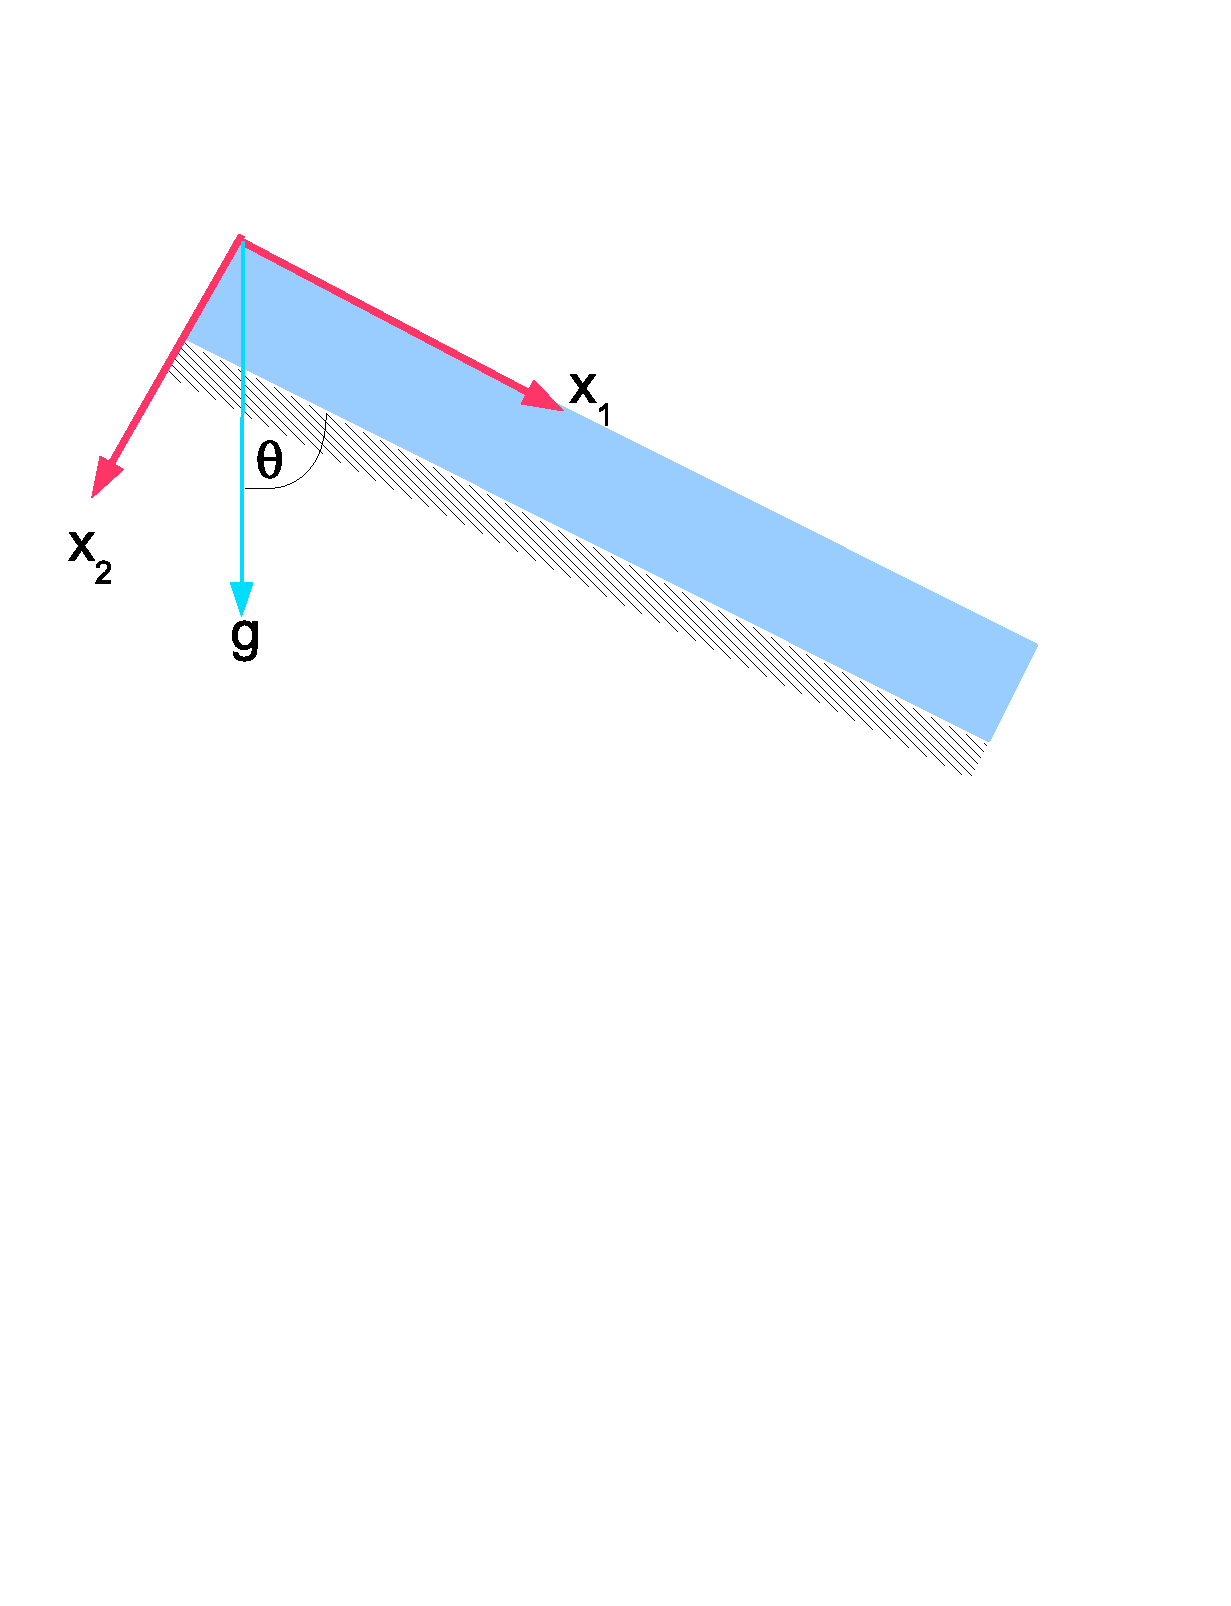
\includegraphics[bb=20 383 545 675, clip]{images/c11-FallingFilm.eps}}}
\end{center}
\caption{Schematic of a film flow problem}
\label{fallfilm}
\end{figure}


Assumptions:
\begin{itemize}
\item Flow is unidirectional. Only $u_1$ needs to be known, $u_2=u_3=0$.
\item Flow is steady state: $\frac{\partial u_1}{\partial t}=0$.
\item Flow is fully developed i.e., it varies only along $x_2$ but not along $x_1$ or $x_3$. $\frac{\partial u_1}{\partial x_1} = 0$ for all $x_1$. 
\item The only driving force for the film to fall is gravity: $\vec{F} = g\cos\theta \hat{x_1} + g\sin\theta \hat{x_2}$.
\end{itemize}


Boundary conditions:
\begin{itemize}
\item Thickness of the film is $\delta$.
\item No slip condition at the bottom of the plane: at $x_2= \delta$, $u_1=0$.
\item At $x_2 = 0$, there is a free surface on which the shear stresses are zero. $\mu \frac{\partial u_1}{\partial x_2}=0$ at $x_2 = 0$.
\end{itemize}


Solution:
Use N-S equation for $u$ and eliminate terms as per the assumptions above.

\begin{equation}
\frac{\partial u_1}{\partial t} + u_1\frac{\partial u_1}{\partial x_1} + u_2\frac{\partial u_1}{\partial x_2} + u_3\frac{\partial u_1}{\partial x_3} = F_1 -  \frac{1}{\rho}\frac{\partial p}{\partial x_1} + \nu \left( \frac{\partial^2 u_1}{\partial x_1^2} + \frac{\partial^2 u_1}{\partial x_2^2} + \frac{\partial^2 u_1}{\partial x_3^2} \right)
\end{equation} 

\begin{equation}
0 =  g \cos\theta + \nu \frac{\partial^2 u_1}{\partial x_2^2} 
\end{equation} 


$$ \frac{\partial^2 u_1}{\partial x_2^2} = -\frac{\rho g \cos\theta}{\mu} $$

$$ u_1 = -\frac{\rho g \cos\theta x^2_2}{2\mu} + C_1 x_2 + C_2 $$

Using the boundary conditions, $C_1 = 0$.

$$ C_2 = \frac{\rho g \cos\theta \delta^2}{2\mu} $$ 
Hence,
$$ u_1 = \frac{\rho \delta^2 g\cos\theta }{2 \mu}\left[1-\left(\frac{x_2}{\delta}\right)^2\right]$$

$$u_1|_{max} = \frac{\rho \delta^2 g\cos\theta}{2 \mu}$$

Using Newton's law $$\sigma_{21} = \tau_{yx} = \mu \frac{\partial u_1}{\partial x_2}$$

$$\tau_{yx} = -\rho g \cos\theta x_2$$


$$\bar{u}_1 = \frac{\int_0^\delta{u_1}dx_2}{\delta} = \frac{\rho \delta^2 g\cos\theta}{3 \mu} = \frac{2}{3} u_1|_{max}$$

If $W$ is the width of the plane, mass flow rate $\dot{M}$ is:

$$ \dot{M} = \rho W \delta \bar{u}_1 = \frac{\rho^2 \delta^3 W g \cos\theta}{3 \mu}$$

The solutions are plotted schematically in figure \ref{fallfilmsol}.

\begin{figure}[h]
\begin{center}
\framebox{\includegraphics[scale=1.0]{images/c11-fallfilmsolfig.ps}}
\end{center}
\caption{Velocity and Stress distribution in a film flow problem}
\label{fallfilmsol}
\end{figure}


Validity:
$$Re = \frac{4\delta \rho \bar{u}_1  }{\mu} \le 25$$ 

%%%%%%%%%%%%%%%%%%%%%%%%%%%%%%%%%%%%%%%%%%%%%%%%%%%%%%%%%%%%%%%%%%%%%%%%%%

\section{Flow between two plates}

\begin{figure}[h]
\begin{center}
\framebox{
\includegraphics[scale=1.0]{images/c11-pchannelfig.ps}
}
\end{center}
\caption{Flow in a channel}
\label{pchannel}
\end{figure}

Figure \ref{pchannel} shows the problem definition. We choose the axes to make the maximum out of the symmetry of the problem.

Assumptions:
\begin{itemize}
\item Flow is unidirectional. Only $u_1$ is to be known, $u_2$ and $u_3$ are zero.
\item Flow is steady state. $\frac{\partial u_1}{\partial t} = 0$.
\item Flow is fully developed. $\frac{\partial u_1}{\partial x_1} = 0$.
\item Pressure gradient is constant $-\frac{\partial p}{\partial x_1} = \frac{p_H - p_L}{L}$
\end{itemize}

Boundary Conditions:
\begin{itemize}
\item No slip condition at bottom layer: at $y=-\delta$, $u_1=0$.
\item No slip condition at top layer: at $y=\delta$, $u_1=0$.
\end{itemize}

Use N-S equation for $u_1$ and eliminate terms as per the assumptions above.

\begin{equation}
\frac{\partial u_1}{\partial t} + u_1\frac{\partial u_1}{\partial x_1} + u_2\frac{\partial u_1}{\partial x_2} + u_3\frac{\partial u_1}{\partial x_3} = F_1 -  \frac{1}{\rho}\frac{\partial p}{\partial x_1} + \nu \left( \frac{\partial^2 u_1}{\partial x_1^2} + \frac{\partial^2 u_1}{\partial x_2^2} + \frac{\partial^2 u_1}{\partial x_3^2} \right)
\end{equation} 

\begin{equation}
\nu \frac{\partial^2 u_1}{\partial x_2^2} = \frac{1}{\rho}\frac{\partial p}{\partial x_1} = \frac{p_L-p_H}{\rho L} 
\end{equation} 
or
\begin{equation}
\frac{\partial^2 u_1}{\partial x_2^2} = -2A 
\end{equation} 

$$A = \frac{p_H-p_L}{2L \mu}$$

$$u_1 = -A x_1^2 + B x_1 + C$$

Using the boundary conditions,

$$\boxed{u_1 = \frac{p_H - p_L}{L} \frac{\delta^2 -x_2^2}{2\mu} }$$

Using Newton's law $$\sigma_{21} = \tau_{21} = \mu \frac{\partial u_1}{\partial x_2}$$

$$\tau_{21} = \frac{p_H - p_L}{2 L} \left( -2x_2 \right)$$

Maximum velocity:
$$\boxed{u_1|_{max} = \frac{p_H - p_L}{L} \frac{\delta^2}{2 \mu}} $$

Average velocity:
$$\boxed{ \bar{u}_1 = \frac{2}{3} u_1|_{max}  = \frac{p_H - p_L}{L} \frac{\delta^2}{3 \mu} }$$


The solutions are plotted schematically in figure \ref{chansol}.

\begin{figure}[h]
\begin{center}
\framebox{
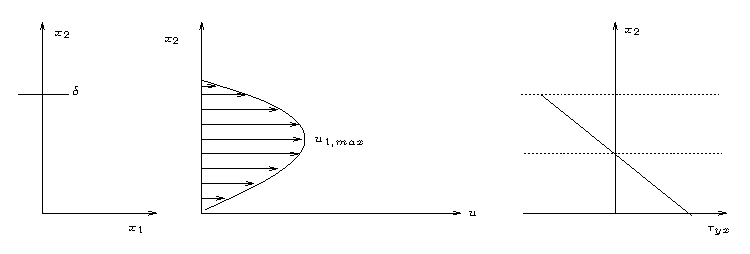
\includegraphics[scale=1.0]{images/c11-chansolfig.ps}
}
\end{center}
\caption{Flow in a channel}
\label{chansol}
\end{figure}

Interpretation of $\tau_{21}$. At $x_2=0$, $\tau_{21} = + A \mu \delta$. Recollecting {\bf convention +} we are using for Newton's law, the shear stress is exerted by the layer at {\em greater} $x_2$ on the layer at {\em lesser} $x_2$ ie., by the liquid on the wall.
At $x_2=\delta$, $\tau_{21} = - A \mu \delta$. The shear stress is exerted by the layer at {\em greater} $x_2$ on the layer at {\em lesser} $x_2$ ie., by the wall on the liquid (thus the negative sign). 

%%%%%%%%%%%%%%%%%%%%%%%%%%%%%%%%%%%%%%%%%%%%%%%%%%%%%%%%%%%%%%%%%%%%%%%%%%

% ------------------------------------------------------------------------------
\begin{figure}[h]
\begin{center}
\frame{
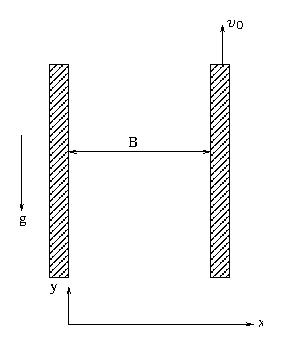
\includegraphics[scale=1.0]{images/c11-mixingfilmfig.ps}
}
\end{center}
\caption{Schematic of a film mixing problem}
\label{MixingFilm}
\end{figure}

\begin{question} 
\item Mixing film: Problem 2B.3 and 2B.4 of~\cite{bls}. An incompressible Newtonian fluid is contained between two long plates of width $W$ = \SI{1}{\metre} (along $z$) and  a distance $B$ = \SI{1}{\mm} apart as shown in figure~\ref{MixingFilm} below. The plate on the right is moved upwards at a velocity $v_0$. Gravity $g$ = \SI{9.81}{\mpss} acts along $y$ axis downwards, density of fluid $\rho$ = \SI{1000}{\kgpmc} and viscosity of fluid \SI{0.01}{\pas}. Assume  the flow is uniaxial, steady state and fully developed. (a) Calculate $v_0$ such that the net volume flow rate across a $y$ plane is zero. (b) What is the ratio of the width of the fluid layer that flows downwards to the width of the fluid layer that flows upwards. (c) Sketch a schematic of the flow field.
\end{question}
\begin{solution}[print]
\end{solution}

% ------------------------------------------------------------------------------

\begin{question} 
Slag film: Problem 2.5 of~\cite{gaskell}. A layer of molten slag of density \SI{2700}{\kgpmc} and viscosity \SI{0.3}{\pascal\second} is being transferred from one reverberatory furnace to another by flow down a plane between the two furnaces inclined at $10^o$ to the horizontal. The plane is \SI{5}{\metre} in width and \SI{5}{\metre} in length and the mass flow rate of the slag is \SI{7.5}{\kilo\gram\per\second}. Neglecting the end effects, calculate (a) thickness of the slag layer (b) average linear flow velocity of the slag and (c) mean residence time of slag on the plane. (d) Fraction of slag that remains on the plane for times equal to or greater than the mean residence time.
\end{question}
\begin{solution}[print]
{\it Answer}: 
(a) \SI{4.77e-3}{\kilo\gram\per\metre\per\second}
(b) \SI{0.116}{\metre\per\second}
(c) \SI{43}{\second}
(d) \num{0.423}
\end{solution}

% ------------------------------------------------------------------------------

\begin{figure}[h]
\label{squeegee}
\begin{center}
\resizebox{!}{3in}{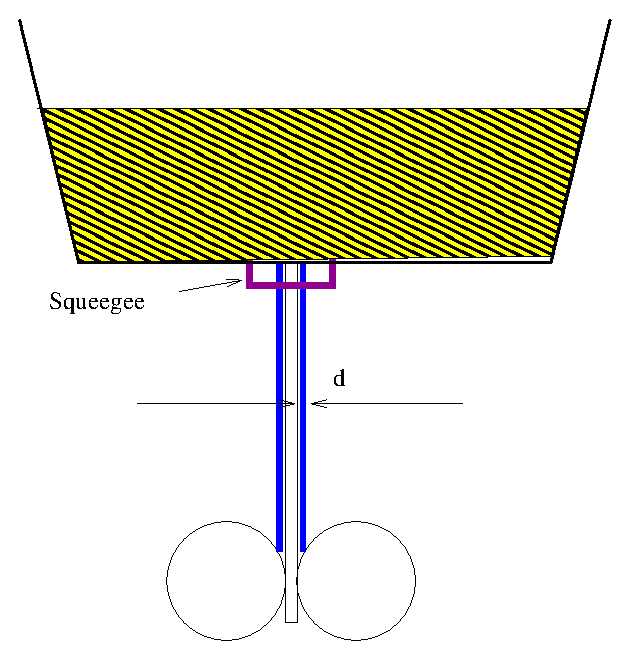
\includegraphics[bb=0 0 287 300, clip]{images/c11-squeegee.eps}}
\end{center}
\caption{Squeegee device}
\end{figure}

\begin{question} 
Squeegee device: A continuous sheet (\SI{1.5}{\metre} wide) of metal is cold-rolled by passing vertically between rolls at a constant speed of \SI{0.3}{\metre\per\second}. Before entering the rolls, the sheet passes through a tank of lubricating oil equipped with a squeegee device that coats both sides of the sheet uniformly as it exits. The amount of oil that is carried through can be controlled by the squeegee device. Determine the mass rate of oil as a function of thickness of oil film that usually range between \SI{0}{\milli\metre} and \SI{0.6}{\milli\metre}. Properties of the lubricating oil: $\rho$ = \SI{962}{\kilo\gram\per\metre\cubed}, $\mu$ = \SI{4.1e-3}{\pascal\second}.
\end{question}
\begin{solution}[print]
\end{solution}

% --------------- end of momcases-planar.tex --------------------------------------------

